\documentclass[12pt]{article}
\usepackage{graphicx,import}
\usepackage[svgnames]{xcolor} 
\usepackage{fancyhdr}
\usepackage{subfig}
\usepackage{hyperref}
\usepackage{enumitem}
\usepackage{cite}
\usepackage[many]{tcolorbox}
\usepackage{listings }
\usepackage[a4paper, total={6in, 8in} , bottom = 25mm , top = 25mm, headheight = 1.25cm , includehead,includefoot,heightrounded ]{geometry}
\usepackage{afterpage}
\usepackage{amssymb}
\usepackage{fancyvrb}
\usepackage{pdflscape}
\usepackage{gensymb}
\usepackage{textcomp}
\usepackage{xecolor}
\usepackage{rotating}
\usepackage{pdfpages}
\usepackage[Kashida]{xepersian}
\usepackage[T1]{fontenc}
\usepackage{tikz}
\usepackage[utf8]{inputenc}
\usepackage{PTSerif} 
\usepackage{seqsplit}

\usepackage[edges]{forest}

\usepackage{listings}
\usepackage{xcolor}

\hypersetup{
	colorlinks   = true, %Colours links instead of ugly boxes
	urlcolor     = blue, %Colour for external hyperlinks
	linkcolor    = blue, %Colour of internal links
	citecolor   = red %Colour of citations
}
 
\definecolor{codegreen}{rgb}{0,0.6,0}
\definecolor{codegray}{rgb}{0.5,0.5,0.5}
\definecolor{codepurple}{rgb}{0.58,0,0.82}
\definecolor{backcolour}{rgb}{0.95,0.95,0.92}
 
\NewDocumentCommand{\codeword}{v}{
\texttt{\textcolor{blue}{#1}}
}
\lstset{language=java,keywordstyle={\bfseries \color{blue}}}

\lstdefinestyle{mystyle}{
    backgroundcolor=\color{backcolour},   
    commentstyle=\color{codegreen},
    keywordstyle=\color{magenta},
    numberstyle=\tiny\color{codegray},
    stringstyle=\color{codepurple},
    basicstyle=\ttfamily\normalsize,
    breakatwhitespace=false,         
    breaklines=true,                 
    captionpos=b,                    
    keepspaces=true,                 
    numbers=left,                    
    numbersep=5pt,                  
    showspaces=false,                
    showstringspaces=false,
    showtabs=false,                  
    tabsize=2
}

\lstset{style=mystyle}

\settextfont[Scale=1.2 ,BoldFont={Bahij Nazanin-Bold.ttf} , ItalicFont = {IRNazaninIranic.ttf}]{Bahij Nazanin-Regular.ttf}
\setlatintextfont[Scale = 1.0]{Garamond}
\DefaultMathsDigits 
\DeclareMathSizes{11}{19}{13}{9} 
%\DeclareMathSizes{12}{14.4}{8}{9}





\newenvironment{changemargin}[2]{%
\begin{list}{}{%
\setlength{\topsep}{0pt}%
\setlength{\leftmargin}{#1}%
\setlength{\rightmargin}{#2}%
\setlength{\listparindent}{\parindent}%
\setlength{\itemindent}{\parindent}%
\setlength{\parsep}{\parskip}%
}%
\item[]}{\end{list}}


\definecolor{foldercolor}{RGB}{124,166,198}

\tikzset{pics/folder/.style={code={%
    \node[inner sep=0pt, minimum size=#1](-foldericon){};
    \node[folder style, inner sep=0pt, minimum width=0.3*#1, minimum height=0.6*#1, above right, xshift=0.05*#1] at (-foldericon.west){};
    \node[folder style, inner sep=0pt, minimum size=#1] at (-foldericon.center){};}
    },
    pics/folder/.default={20pt},
    folder style/.style={draw=foldercolor!80!black,top color=foldercolor!40,bottom color=foldercolor}
}

\forestset{is file/.style={edge path'/.expanded={%
        ([xshift=\forestregister{folder indent}]!u.parent anchor) |- (.child anchor)},
        inner sep=1pt},
    this folder size/.style={edge path'/.expanded={%
        ([xshift=\forestregister{folder indent}]!u.parent anchor) |- (.child anchor) pic[solid]{folder=#1}}, inner xsep=0.6*#1},
    folder tree indent/.style={before computing xy={l=#1}},
    folder icons/.style={folder, this folder size=#1, folder tree indent=3*#1},
    folder icons/.default={12pt},
}

\begin{document}


%%% title pages
\begin{titlepage}
\begin{center}
        
\vspace*{0.7cm}


\includegraphics[width=0.4\textwidth]{sharif1.png}\\
\vspace{0.5cm}
\textbf{ \Huge{\emph ‌اندازه‌گیری و کنترل کامپیوتری} }\\
\vspace{0.5cm}
\textbf{ \Large{ تمرین چهارم} }
\vspace{0.2cm}
       
 
      \large \textbf{دانشکده مهندسی کامپیوتر}\\\vspace{0.2cm}
    \large   دانشگاه صنعتی شریف\\\vspace{0.2cm}
       \large   ﻧﯿﻢ سال دوم 00-99 \\\vspace{0.2cm}
      \noindent\rule[1ex]{\linewidth}{1pt}
استاد:\\
    \textbf{{جناب آقای دکتر همت‌یار}}


    \vspace{0.15cm}
نام و نام خانوادگی:\\

       
    \textbf{{امیرمهدی نامجو - 97107212}}
\end{center}
\end{titlepage}
%%% title pages


%%% header of pages
\newpage
\pagestyle{fancy}
\fancyhf{}
\fancyfoot{}
\cfoot{\thepage}
\chead{تمرین چهارم}
\rhead{
\includegraphics[width=0.1\textwidth]{sharif.png}}
\lhead{امیرمهدی نامجو}
%%% header of pages

\KashidaOff


\section*{سوال 3}

$$150 \degree C = (150 + 273.15) K= 423.15 K$$

$$150 \degree C = (\frac{9}{5}150 + 32) \degree F = 302 \degree F$$


\section*{سوال 6}
 
 $$\frac{9}{5} 350 + 32 = 550 \degree F$$
 $$\frac{9}{5} 550 + 32 = 1022 \degree F$$

\section*{سوال 9}
 
 برای تخمین خطی
 
 $$\alpha_0 = \frac{1}{R(T_0)} \frac{R_2 - R_1}{T_2 -T_1} \alpha_0$$
 
 در این جا
 $$T_0 = 115 \degree C , T_1 = 100 \degree C , T_2 = 130 \degree C$$
 
 $$R_0 = 589.48 \Omega , R_1 = 573.40 \Omega , R_2 = 605.52 \Omega$$
 
 $$\alpha_0 = \frac{1}{589.48}\frac{(605.52 - 573.40)}{130 -100} = 0.0018 \frac{1}{\degree C}$$
 
 
 $$R(T) = 589.48[1+0.0018(T-115)]$$
 
 
 برای تخمین Quadratic:
 
 $$R(T) = R(T_0) [1+\alpha_1 \Delta T + \alpha_2 (\Delta T)^2]$$
 
 مقادیر را برای $100 \degree C$ و $130 \degree C$ در نظر می‌گیریم و براساس آن‌ها دو معادله دو مجهول تشکیل می‌دهیم:
 
 $$573.40 = 589.48 [1 -15 \alpha_1 + 225 \alpha_2]$$
 $$605.52 = 589.48[1 + 15 \alpha_1  +225 \alpha_2]$$
 
 
 $$-15 \alpha_1 + 225 \alpha_2 = -0.027278$$
 $$15 \alpha_1 + 225 \alpha_2 = 0.027278$$
 
 $$\alpha_1 = 1.82 \times 10^3 \frac{1}{\degree C} , \alpha_2 = -1.51 \times 10^{-7} (\frac{1}{\degree C})^2$$
 
 $$R(T) = 589.48[1+0.00182 \Delta T + 1.51 \times 10^{-7} (\Delta T)^2]$$
 
 در مورد خطا برای نقطه $105 \degree C$ بررسی می‌کنیم که مقدار مقاومت در آن
 $578.77 \Omega$
 است:
 
 $$R_{Linear} = 589.48[1 + 0.0018 (105 - 115)] =  578.87$$
 
 که خطای $0.17$ درصدی نسبت به مقدار واقعی دارد و از آن بیش تر است.
 
 $$R_{Quadratic} = 589.48[1 + 0.00182 (105 -115) -1.51  \times 10^{-7} \times (105 -115)^2 = 578.74 \Omega ]$$
 
 که خطای $0.005$ درصدی دارد و به این میزان از عدد واقعی کمتر است.
 
\newpage 
\section*{سوال 12}
 
 برای این که اثر خودگرمایی را به $0.1 \degree C$ برسانیم داریم:
 
 $$P = P_D \delta T = (5 mW / \degree C) (0.1 \degree C) = 500 \mu W$$
 همچنین داریم:
 
 $$I = \sqrt{P/R} = \sqrt{\frac{5\times 10^-4}{3.5 \times 10^3}} = 378 \mu A$$
 
 $$I = V/{R + R_{TH}} \rightarrow 378 \times 10^{-6} = 10/(R + 3500) \rightarrow R = 22955 \Omega \approx 23 k \Omega$$
 
 با توجه به این که گفته شده شیب خط 
 $-10\%/\degree C$
 است یعنی در $21$ درجه
 $3.5 - 0.35 = 3.15 k\Omega$
 و در $19$ درجه مقاومت
 $3.5 + 3.5 = 3.85 k\Omega$
 است.
 
 برای بدست آوردن ولتاژ تقسیم کننده داریم:
 
 $$V_D = 10 \frac{R_{TH}}{23 k \Omega + R_{TH}}$$
 
 $$T=20\degree C \rightarrow V_D = 1.32 V$$
 
 $$T=21\degree C \rightarrow V_D = 1.20 V$$
 
 $$T=19\degree C \rightarrow V_D = 1.43 V$$
 
\newpage
\section*{سوال 15}

جدول Type-S در شکل زیر آمده است  (تصویر قابل زوم کردن است):

\begin{center}
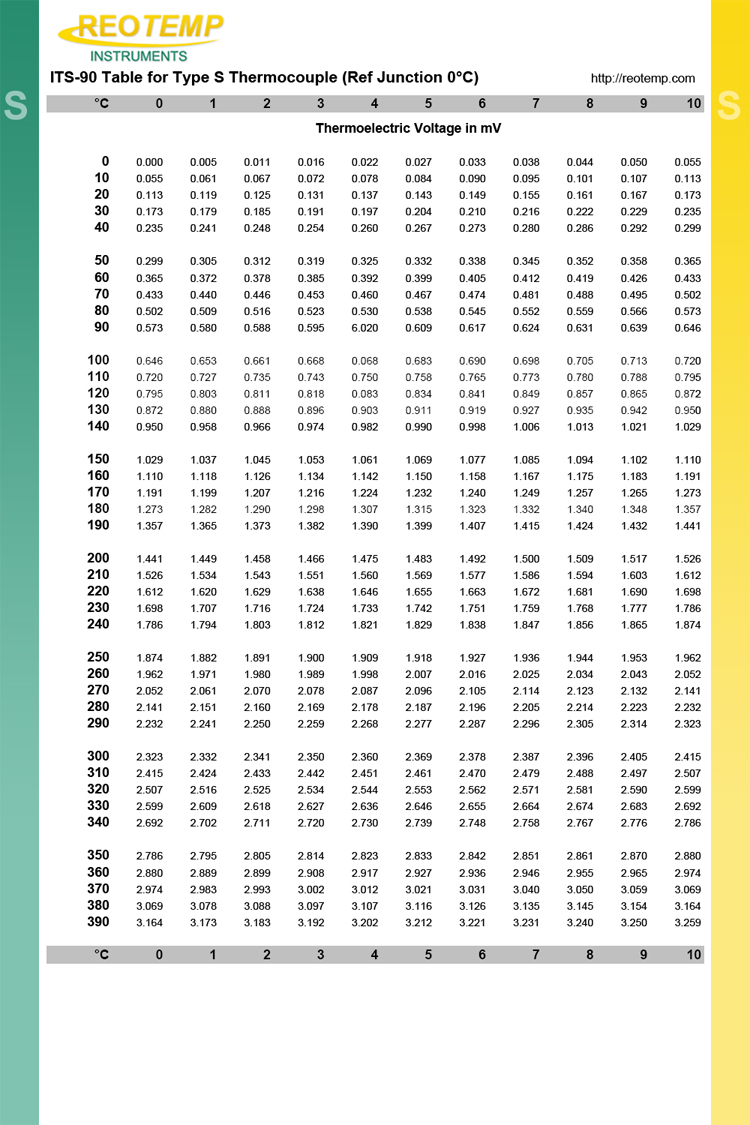
\includegraphics[width = 0.3 \textwidth]{images/1.jpg}
\end{center}


\begin{center}
	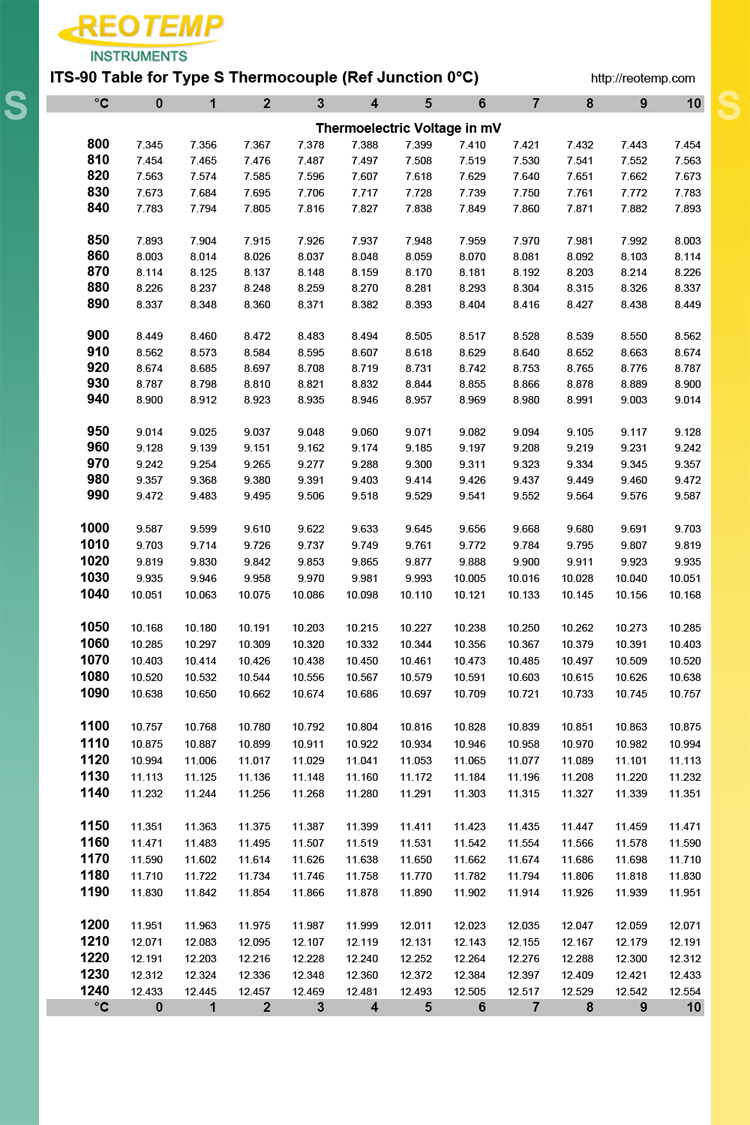
\includegraphics[width = 0.3 \textwidth]{images/2.jpg}
\end{center}


با توجه به رفرنس داده شده، باید تصحیح مربوط به آن را اعمال کنیم. برای $21$ درجه رفرنس $0.119mV$ است. البته از طریق درون یابی روی نمودار هم می‌توان به این عدد رسید.

پس در اصل ولتاژ را باید
$$V_c = 12.120 + 0.119 = 12.239 mV$$

در نظر بگیریم. این عدد بین $1223$ و $1224$ در نمودار است. برای تعیین مقدار دقیق آن داریم:

$$T(12.239 mV) = 1223 + \frac{1224-1223}{12.240-12.228} (12.239 - 12.228) = 1223.917 \approx 1223.92 \degree C $$



\newpage
\section*{سوال 18}

جدول ترموکوپل نوع K در شکل زیر آمده است (تصویر قابل زوم کردن است):
 
 \begin{center}
 	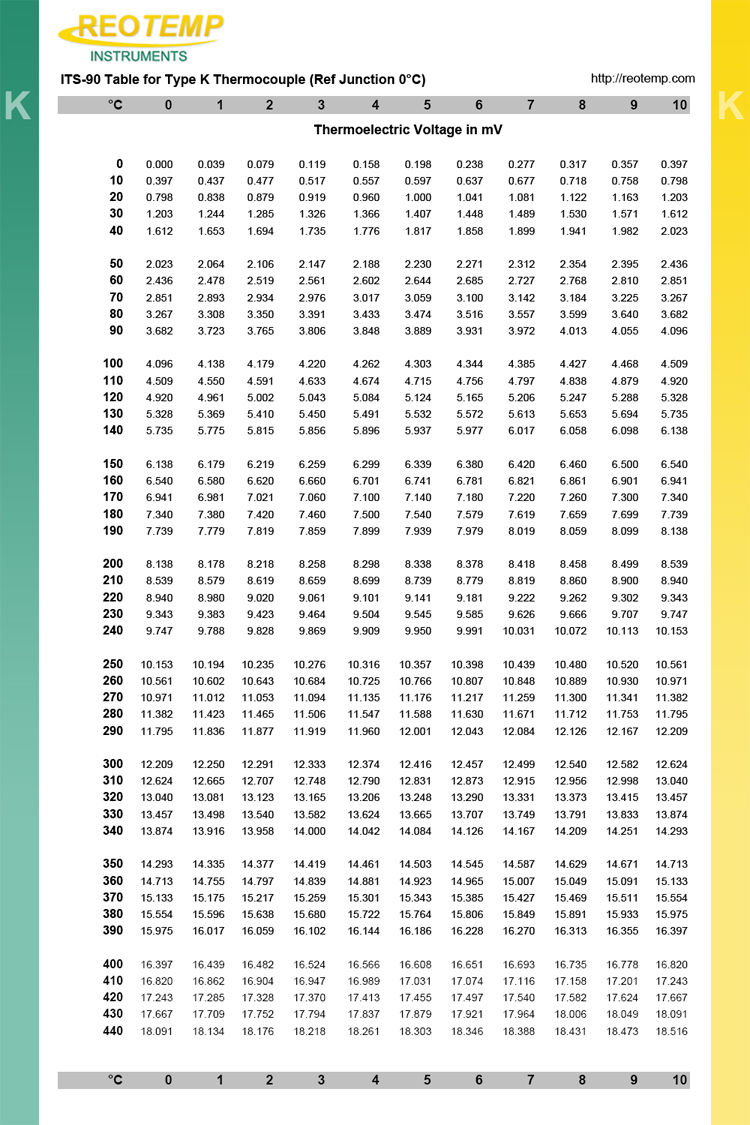
\includegraphics[width = 0.25 \textwidth]{images/3.jpg}
 \end{center}

 
\begin{center}
	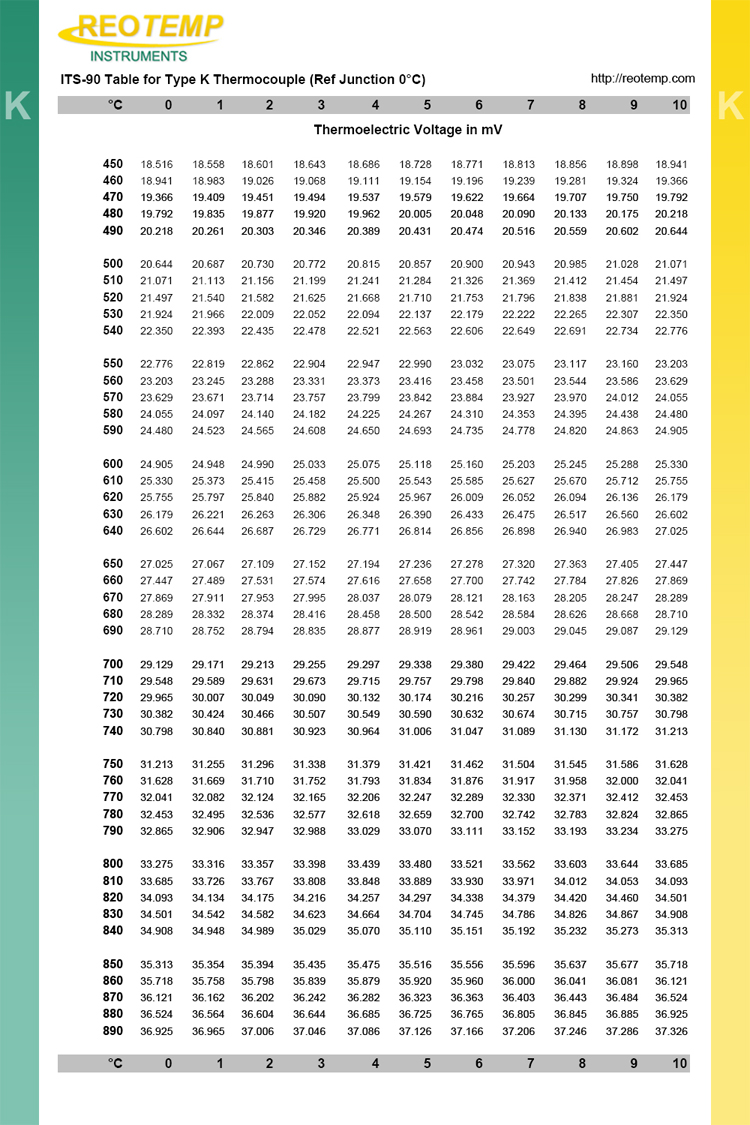
\includegraphics[width = 0.25 \textwidth]{images/4.jpg}
\end{center}


$$70 \degree F = \frac{5}{9} (70 -32) = 21.1 \degree C$$

$70$ درجه فارنهایت برابر حدودا $21$ درجه سلسیوس است. برای $21$ درجه رفرنس $0.838$ میلی‌ولت است.  مقدار مربوط به $700$ درجه هم $29.129$ میلی‌ولت است. در نتیجه ولتاژی که در این جا داریم:
$$29.129 - 0.838 = 28.291 mV$$
است.

برای تولید ولتاژ $1.5V$ داریم:

$$1.5V / 28.291 mV = 53.0204 $$

یعنی حدودا $53$ یا $54$ ترموکوپل به صورت سری نیاز داریم.

\newpage
\section*{سوال 21}


داریم:

$$70 \degree F = \frac{5}{9} (70 -32) = 21.1 \degree C$$


$$200 \degree F = \frac{5}{9} (200 -32) = 93.3 \degree C$$

\begin{center}
	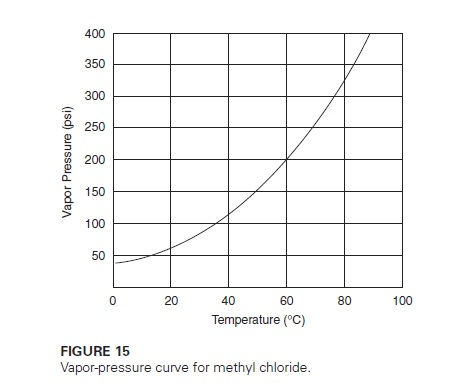
\includegraphics[width = 0.5 \textwidth]{images/5.jpg}
\end{center}

با توجه به شکل $15$ کتاب در صفحه $222$ مقدار نظیر برای $70$ درجه فارنهایت حدود $60psi$ و برای $200$ درجه فارنهایت حدودا مقداری بیش تر از $400$ یعنی $410 psi$ است. باید توجه کرد که در شکل مقدار مربوط به $200$ در نمودار قرار نگرفته است و در نتیجه با توجه به نزدیکی نقطه آخر نمودار به $400$ می‌توان متوجه این شد که احتمالا باید در حدود $410psi$ برای $200$ فارنهایت معادل $93.3$ درجه سلسیوس داشته باشیم.


\newpage
\section*{سوال 24}


برای ترموکوپل نوع $k$ داریم:

$$200 \degree C \rightarrow 8.13 mV$$

$$350 \degree C \rightarrow 14.29 mV$$

همچنین رفرنس ADC که داریم $2.5$ ولت است. ولتاژ گذار از FE به FF به صورت

$$V_{ADC} =\frac{255}{256} V_{ref} = 2.5 - 2.5/256 = 2.49 V$$
است. در نتیجه باید $8.13mv$ نظیر به $0$ و $14.29mV$ نظیر به $2.49V$ بشود.


$$0 = 0.00813 m + V_0$$
$$2.49 = 0.01429 m + V_0$$

در نتیجه

$$m = 404.2 , V_0 = -3.286V = (404.2)(-0.00813)$$


شکل نهایی مدار مورد نظر بدین صورت است:


\begin{center}
	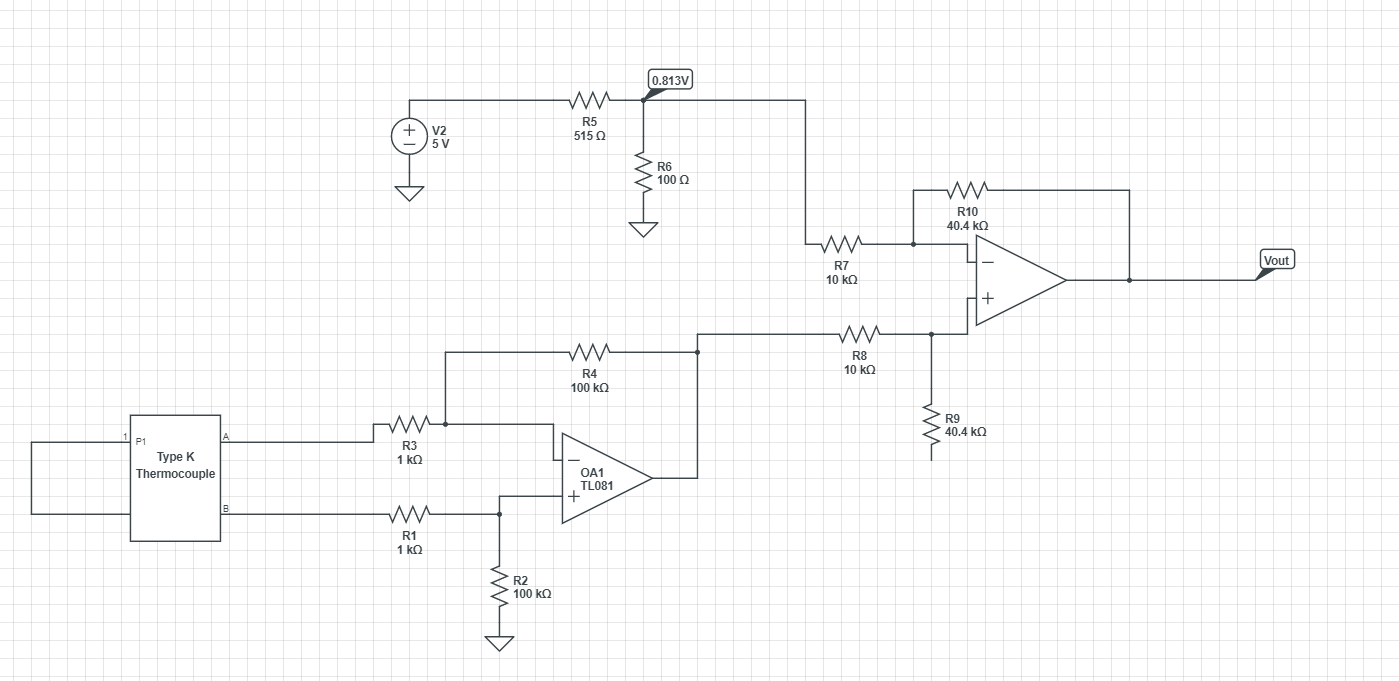
\includegraphics[width = 1.0 \textwidth]{images/6.png}
\end{center}



خروجی این مدار وارد ADC می‌شود.

\newpage
\section*{سوال 27}

با توجه به صورت سوال و اعداد گفته شده برای ADC یعنی هر بیت باید معادل با $1\degree F$ باشد. باید محدوده خودگرمایی را حدود $0.1$ این مقدار نگه داریم. $0.1\degree F$ برابر $0.056 \degree C$ است. پس باید
$$P<P_D \delta T = (0.056)(0.005) = 0.28 mW$$
باشد. داریم:
$$I = sqrt{P/R} =\sqrt{0.000028/5000} = 240 \mu A$$

یعین جریان نباید از این مقدار بیش تر بشود.


از سوی دیگر برای ADC داریم:

$$90 \degree F: V_L = 5 \frac{90}{256} = 1.758V $$
$$110 \degree F: V_H = 5 \frac{110}{256} = 2.148 V$$

همچنین باید مقاومت را در $110\degree F$ تعیین کنیم که داریم:

$$R_{110 \degree F} = 5000 - (8 \Omega / \degree C)(110 \degree F - 90\degree F)(5/9) = 4911 \Omega$$

از آن جایی که جریان باید کمتر از $240$ میکرو آمپر باشد، ترمیستور را در شاخه فیدبک منفی یک آپ‌امپ قرار داده و به کمک مرجع $15V-$ ای جریان $100$ میکرو آمپری ایجاد می‌کنیم که مقدار جریان از عدد گفته شده بالاتر نرود.

با توجه به این شرایط، باید ولتاژ جلوی آپ آمپ که در شکل با $V_a$ نمایش داده شده را بدست آوریم:

$$90 \degree F: V_a = -(5000 \Omega) \times (- 100 \mu A) = 0.500 V$$
$$110 \degree F: V_a = -(4911 \Omega) \times (-100 \mu A) = 0.4911$$

در نتیجه با توجه به ولتاژ هایی که برای ADC بدست آوردیم داریم:

$$1.758 = m(0.5000) + V_0$$
$$2.148 = m (0.4911) + V_0$$

با حل دستگاه داریم:

$$m = -43.82 , V_0 = 23.67$$

یعنی معادله نهایی:
$$43.82(0.5401 - V_s)$$

است. در نتیجه مدار زیر را تشکیل می دهیم:




\begin{center}
	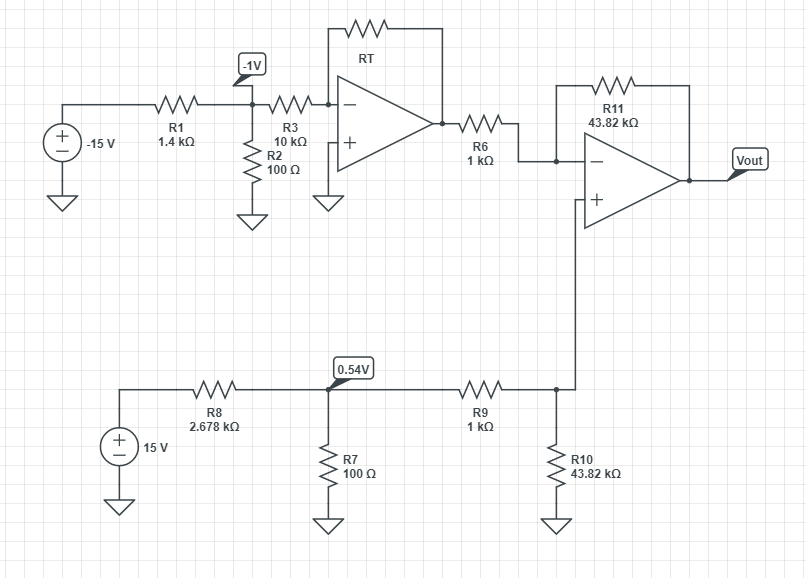
\includegraphics[width = 1.0 \textwidth]{images/7.png}
\end{center}

\newpage 
\section*{سوال 30}

بازه بین $50$ تا $100$ درجه با وضوح $0.1$ معادل $500$ واحد است. در نتیجه نیاز به حداقل $9$ بیت در ADC داریم و از آن جایی که $9$ بیت عدد رایجی برای ADC ها نیست، از ADC تک قطبی $10$ بیتی استفاده می کنیم. ولتاژ رفرنس را هم $5V$ می گیریم.  باید ابتدا مقاومت‌های مربوطه را بدست آوریم:

$$R_{50\degree C} = 306.5[1 + 0.0041(50-20)] = 344.2 \Omega$$
$$R_{100 \degree C} = 306.5 [1 + 0.0041 (100 -20)] = 407.0 \Omega$$


برای این سوال از یک Bridge استفاده می کنیم. مدار های دیگر هم قابل استفاده هستند. باید اثر خودگرمایی را کمتر از $0.01 \degree C$ نگه داریم که از وضوح $0.1\degree C$ مطمئن باشیم.

$$P_Max = (0.030)(0.01) = 0.3 mW$$

$$P = V^2 / R \rightarrow V= \sqrt{PR} = \sqrt{0.3 \times 344.2} = 0.3 V$$

بنابراین باید در دمای $50$ درجه ولتاژ دو سر RTD برابر $0.3$ ولت باشد و در این حالت پل را null کنیم. RTD را به عنوان $R_3$ قرار می دهیم و $R4=1k\Omega$ می گیریم. در این صورت:

$$R_1 = \frac{5-0.3}{(0.3-0)/344.2} = 5393 \Omega$$

$$R_2 = \frac{5-0.3}{(0.3-0)/1000} = 15.7 k\Omega$$

با توجه به این موارد بایید توجه کنیم که در $100\degree C$ ولتاژ سر سمت راست پل در شکل همان $0.3$ خواهد بود ولی ولتاژ سر سمت چپ 
$5 \frac{407}{407+5393} = 0.3509 V$
خواهد بود و در نتیجه اختلاف ولتاژ
$$\Delta V = 0.3509 - 0.3 - 0.0509 V$$
خواهیم داشت.

از آن جایی که ورودی ADC در حالت بیشینه باید
$(1023/1024) \times 5V = 4.995$
باشد، باید از تقویت کننده با بهره
$\frac{4.995 / 0.0509} = 98.13$ 
استفاده کنیم. در نهایت معادله کلی به صورت
$$V_{out} = 98.13 (5 \frac{R}{R+5393} - 0.3)$$
خواهد بود که $V_{out}$ خروجی مدار شکل زیر و ورودی ADC خواهد بود.






\begin{center}
	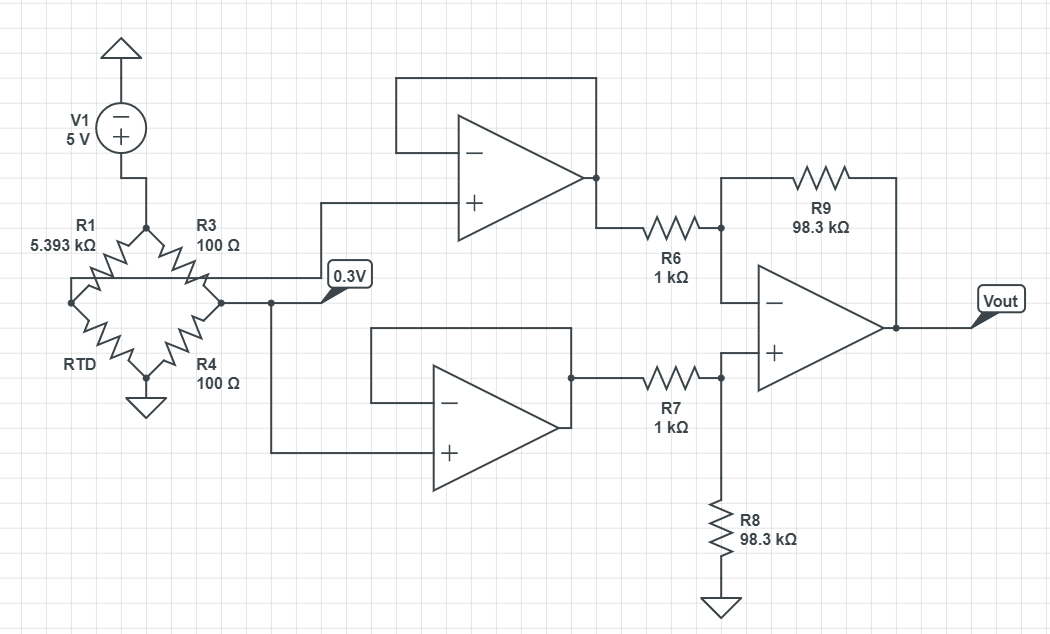
\includegraphics[width = 1.0 \textwidth]{images/8.png}
\end{center}

\end{document}



